\documentclass[tikz,border=10pt]{standalone}
\usepackage{tikz}
\usetikzlibrary{shapes.geometric, arrows.meta, positioning, calc}

\tikzstyle{devopsbox} = [rectangle, minimum width=3.5cm, minimum height=1.2cm, text centered, draw=black, fill=blue!15]
\tikzstyle{arrow} = [thick, ->, >=Stealth]
\tikzstyle{feedback} = [thick, ->, >=Stealth, dashed, red]

\begin{document}

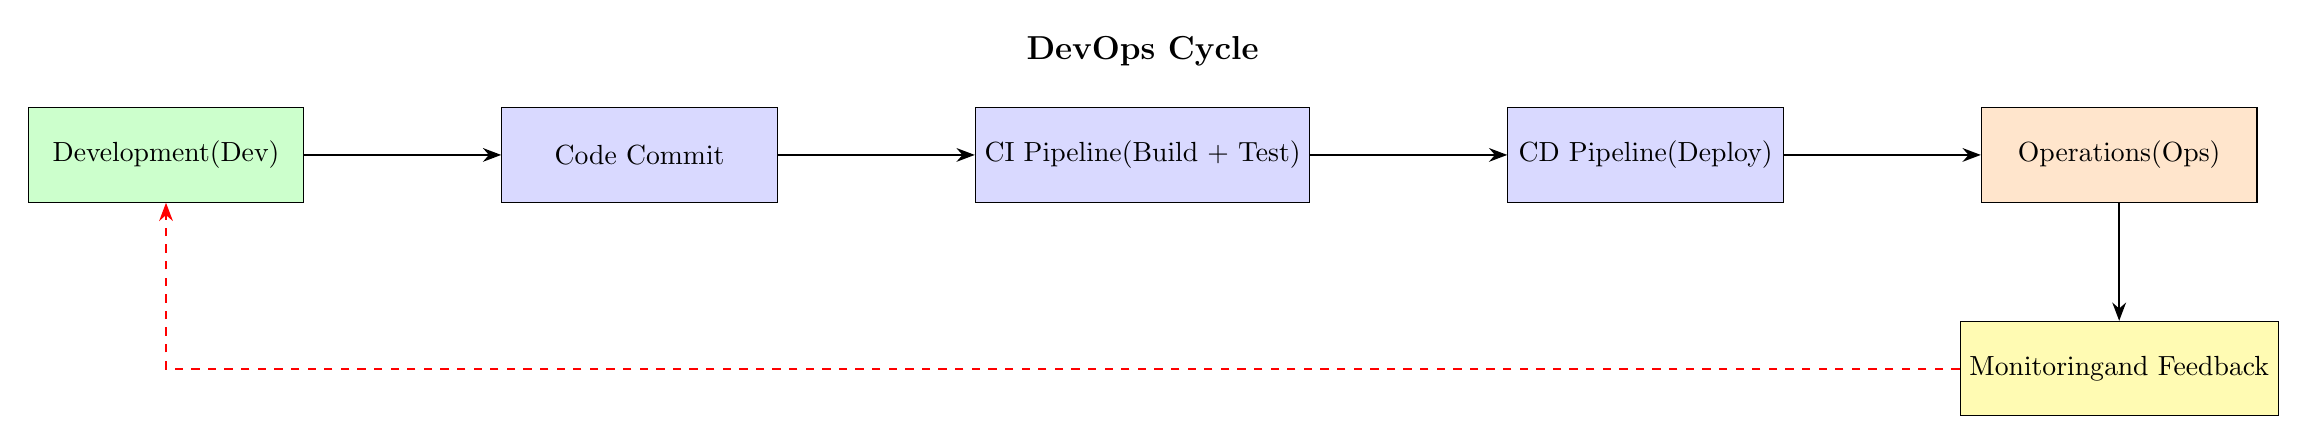
\begin{tikzpicture}[node distance=1.5cm and 2.5cm]

% Nodes
\node (dev) [devopsbox, fill=green!20] {Development\\(Dev)};
\node (code) [devopsbox, right=of dev] {Code Commit};
\node (ci) [devopsbox, right=of code] {CI Pipeline\\(Build + Test)};
\node (cd) [devopsbox, right=of ci] {CD Pipeline\\(Deploy)};
\node (ops) [devopsbox, right=of cd, fill=orange!20] {Operations\\(Ops)};
\node (monitor) [devopsbox, below=of ops, fill=yellow!30] {Monitoring\\and Feedback};

% Arrows
\draw [arrow] (dev) -- (code);
\draw [arrow] (code) -- (ci);
\draw [arrow] (ci) -- (cd);
\draw [arrow] (cd) -- (ops);
\draw [arrow] (ops) -- (monitor);
\draw [feedback] (monitor.west) -| (dev.south);

% Labels
\node at ($(dev)!0.5!(ops)$) [above=1cm, font=\bfseries\large] {DevOps Cycle};

\end{tikzpicture}

\end{document}
